\begin{figure}
  \begin{subfigure}{0.48\columnwidth}
    \resizebox{\textwidth}{!}{%
      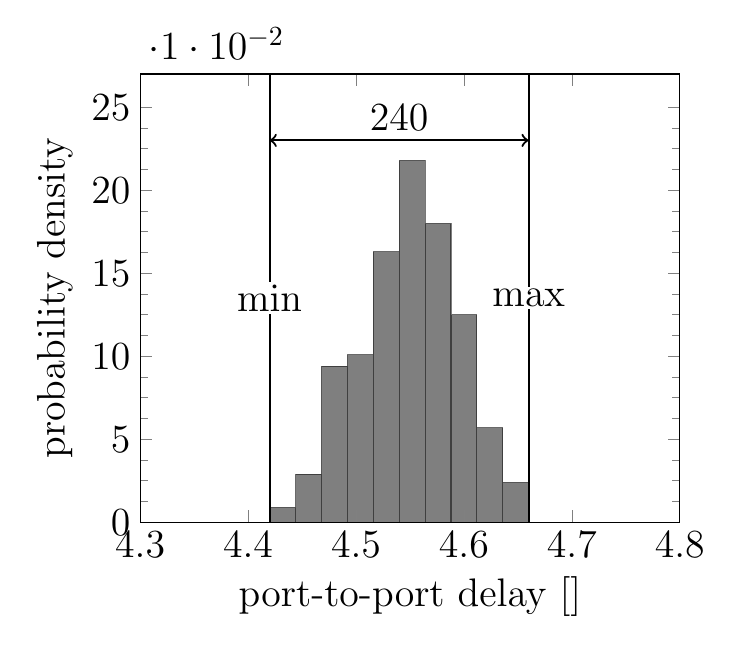
\begin{tikzpicture}
	  \begin{axis}[
	      ymin=0, ymax=0.27,
	      xmin=4.3,xmax=4.8,
	      minor y tick num = 3,
	      scaled y ticks=real:0.01,
	      area style,
	      xlabel={port-to-port delay [\si{\us}]},
	      ylabel={probability density},
	      font=\Large,
	      ]
	      \addplot+[ybar interval,mark=no,black,fill=black,semitransparent] plot coordinates { 
		  (4.42, 0.009) (4.444,0.029) (4.468,0.094) (4.492,0.101) (4.516,0.163) (4.54,0.218) (4.564,0.18) (4.588,0.125) (4.612,0.057) (4.636,0.024) (4.66,0)  
	      };
	      \draw (axis cs:4.42,0) edge[thick] node[inner sep=1pt,fill=white,pos=0.5] {min} (axis cs:4.42,0.27);
	      \draw (axis cs:4.66,0) edge[thick] node[inner sep=1pt,fill=white,pos=0.5] {max} (axis cs:4.66,0.27);
	      \draw (axis cs:4.42,0.23) edge[thick,<->] node[above] {$\qty{240}{\ns}$} (axis cs:4.66,0.23);
	  \end{axis}
      \end{tikzpicture}
    }
    \caption{Wired TSN bridge}
  \end{subfigure}
  \hfill
  \begin{subfigure}{0.48\columnwidth}
    \resizebox{\textwidth}{!}{%
      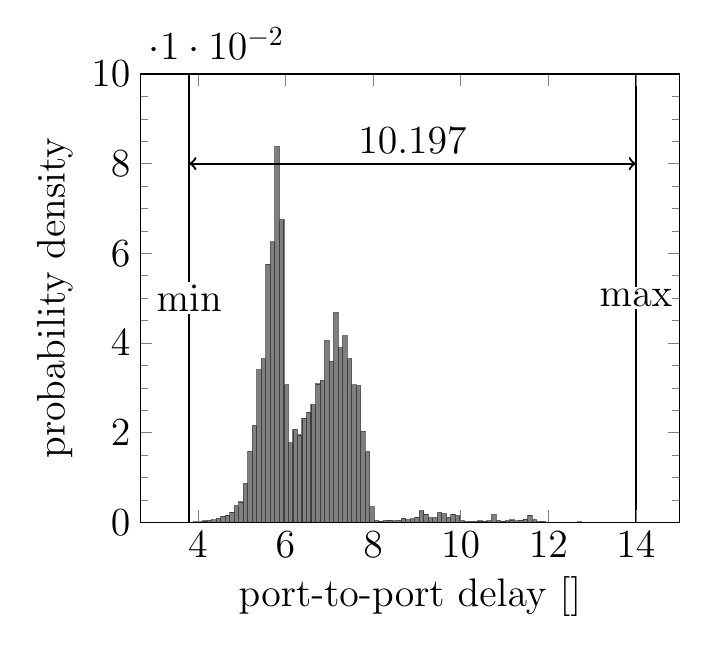
\begin{tikzpicture}
	  \begin{axis}[
	      ymin=0, ymax=0.1,
	      xmax=15,
	      minor y tick num = 3,
	      scaled y ticks=real:0.01,
	      area style,
	      xlabel={port-to-port delay [\si{\ms}]},
	      ylabel={probability density},
	      font=\Large,
	      ]
	      \addplot+[ybar interval,mark=no,black,fill=black,semitransparent] plot coordinates { 
		  (3.803,1e-05) (3.906,0.00011) (4.009,0.00011) (4.112,0.00029) (4.215,0.00041) (4.318,0.00055) (4.421,0.00088) (4.524,0.00136) (4.627,0.00161) (4.73,0.00224) (4.833,0.00372) (4.936,0.00452) (5.039,0.00866) (5.142,0.01582) (5.245,0.02163) (5.348,0.03399) (5.451,0.03653) (5.554,0.0576) (5.657,0.06254) (5.76,0.08382) (5.863,0.06751) (5.966,0.03065) (6.069,0.01778) (6.172,0.0207) (6.275,0.01947) (6.378,0.02322) (6.481,0.02457) (6.584,0.02623) (6.687,0.03085) (6.79,0.03164) (6.893,0.0405) (6.996,0.03587) (7.099,0.04674) (7.202,0.03896) (7.305,0.0416) (7.408,0.03652) (7.511,0.03066) (7.614,0.03047) (7.717,0.02029) (7.82,0.01577) (7.923,0.00345) (8.026,0.00041) (8.129,0.00026) (8.232,0.00044) (8.335,0.00048) (8.438,0.00033) (8.541,0.00041) (8.644,0.00093) (8.747,0.00057) (8.85,0.00075) (8.953,0.00116) (9.056,0.00262) (9.159,0.0018) (9.262,0.00104) (9.365,0.00103) (9.468,0.00219) (9.571,0.00187) (9.674,0.00109) (9.777,0.00183) (9.88,0.00148) (9.983,0.00039) (10.086,0.00017) (10.189,0.0002) (10.292,0.0002) (10.395,0.00028) (10.498,0.00024) (10.601,0.0003) (10.704,0.00171) (10.807,0.00045) (10.91,0.00027) (11.013,0.00037) (11.116,0.0005) (11.219,0.00033) (11.322,0.00046) (11.425,0.0007) (11.528,0.00158) (11.631,0.00057) (11.734,0.00023) (11.837,0.0002) (11.94,5e-05) (12.043,1e-05) (12.146,0.0) (12.249,1e-05) (12.352,1e-05) (12.455,0.0) (12.558,3e-05) (12.661,6e-05) (12.764,1e-05) (12.867,1e-05) (12.97,1e-05) (13.073,1e-05) (13.176,1e-05) (13.279,0.0) (13.382,0.0) (13.485,4e-05) (13.588,0.0) (13.691,2e-05) (13.794,0.0) (13.897,2e-05) (14.0,0.0) 
	      };
	      \draw (axis cs:3.803,0) edge[thick] node[inner sep=1pt,fill=white,pos=0.5] {min} (axis cs:3.803,0.1);
	      \draw (axis cs:14,0) edge[thick] node[inner sep=1pt,fill=white,pos=0.5] {max} (axis cs:14,0.1);
	      \draw (axis cs:3.803,0.08) edge[thick,<->] node[above] {$\qty{10.197}{\ms}$} (axis cs:14,0.08);
	  \end{axis}
      \end{tikzpicture}
    }
    \caption{Logical 5G-TSN bridge}
  \end{subfigure}
  \caption{Packet delay characteristics, measured by \cite{downlink_example_histogram}.} \label{fig:delays}
\end{figure}

